%\documentclass[a4paper, 12pt]{report}
\documentclass[12pt,a4paper,openany]{abntex2}

\usepackage[T1]{fontenc}
%\usepackage[latin1]{inputenc}
%\usepackage[verbose,left=30mm,right=20mm,top=30mm,bottom=30mm]{geometry}
%\usepackage{txfonts}
\usepackage[brazil]{babel}
\usepackage{pdfpages}
%\usepackage[authoryear]{natbib}
%\usepackage{appendix}
%\usepackage{setspace}
%\usepackage{url}
%\usepackage{hyperref}
%\usepackage{color}
\usepackage[utf8]{inputenc}
\usepackage{placeins}
\usepackage{float}

\autor{Leonardo Mendonça de Araujo \and \\ Lucas Bagatini do Nascimento \and \\ Mário Muramatsu Júnior}
\titulo{RELATÓRIO DE FINAL: IDENTIFICADOR DE SINAIS TRIFÁSICOS}
\data{2018} 
\local{Rio Claro, São Paulo}
\preambulo{Monografia apresentada ao curso de Ciências da Computação, como requisito parcial para a obtenção do Título de Bacharel em Ciências da Computação, Instituto de Geociências e Ciências Exatas da Universidade Estadual Paulista}
\orientador{Mario Roberto da Silva}
\tipotrabalho{monografia}

\begin{document}
	
\imprimircapa	
\imprimirfolhaderosto

\clearpage
\cleardoublepage
\cleardoublepage

\pagenumbering{arabic}
\setcounter{page}{3}

\tableofcontents
\clearpage{\pagestyle{empty}\cleardoublepage}
	
\chapter{Introdução}

\section{Sistemas Elétricos Polifásicos}

Naturalmente, sistemas elétricos funcionando em corrente alternada possuem picos e vales de tensão e, consequentemente, picos e vales de potência. A fim de mitigar esta ineficiência intrínseca, pode-se montar um sistema polifásico, ou seja, um sistema que fornece energia elétrica através de três ou mais condutores energizados.

As figuras ~\ref{fig:sinal-bifasico} e ~\ref{fig:sinal-trifasico} ilustram o comportamente da tensão em sistemas bifásicos e trifásicos, respectivamente. É trivial perceber que sistemas polifásicos são capazes de fornecer tensão e potência de maneira mais constante e sem necessitar de altos picos em cada uma de suas fases.

\begin{figure}[!htp]
	\centering
	\fbox{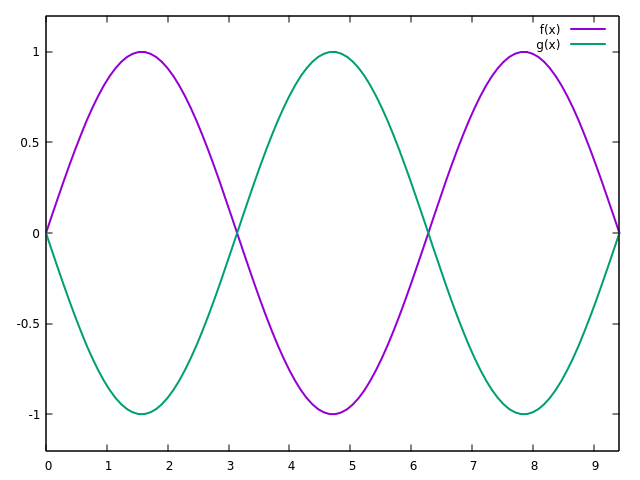
\includegraphics[width=16cm]{./images/Bifasico.png}}
		\caption{Exemplo de sistema Bifásico}
	\label{fig:sinal-bifasico}
\end{figure}

\begin{figure}[!htp]
	\centering
	\fbox{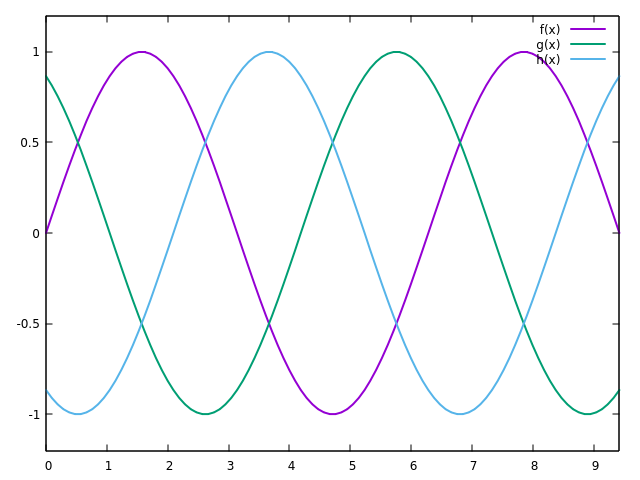
\includegraphics[width=16cm]{./images/Trifasico.png}}
		\caption{Exemplo de sistema Trifásico}
	\label{fig:sinal-trifasico}
\end{figure}

Um sinal trifásico, como da Figura ~\ref{fig:sinal-trifasico}, assim como outras variações de sinais polifásicos, são criados nos geradores; originados dos motores de indução polifásicos desenvolvidos concomitantemente por Galileo Ferraris, Nikola Tesla e Mikhail Dolivo-Dobrovolsky. Um gerador alternador trifásico é composto por um núcleo magnético assim como qualquer outro alternador, e seu estator é composto de bobinas ligadas aos três condutores ao invés de dois, como em um alternador simples. Conforme o rotor gira, este excita os elétrons livres nas bobinas dentro de seu campo magnético, criando corrente alternada. Existe, portanto, uma relação de proporcionalidade direta entre o espaçamento das bobinas e às distâncias das fases em cada um dos condutores.

FONTE DESSA PORRA: Ion Boldea, Syed Abu Nasar, The Induction Machine Handbook - CRC Press, 2002, page 2


\begin{figure}[!htp]
	\centering
	\fbox{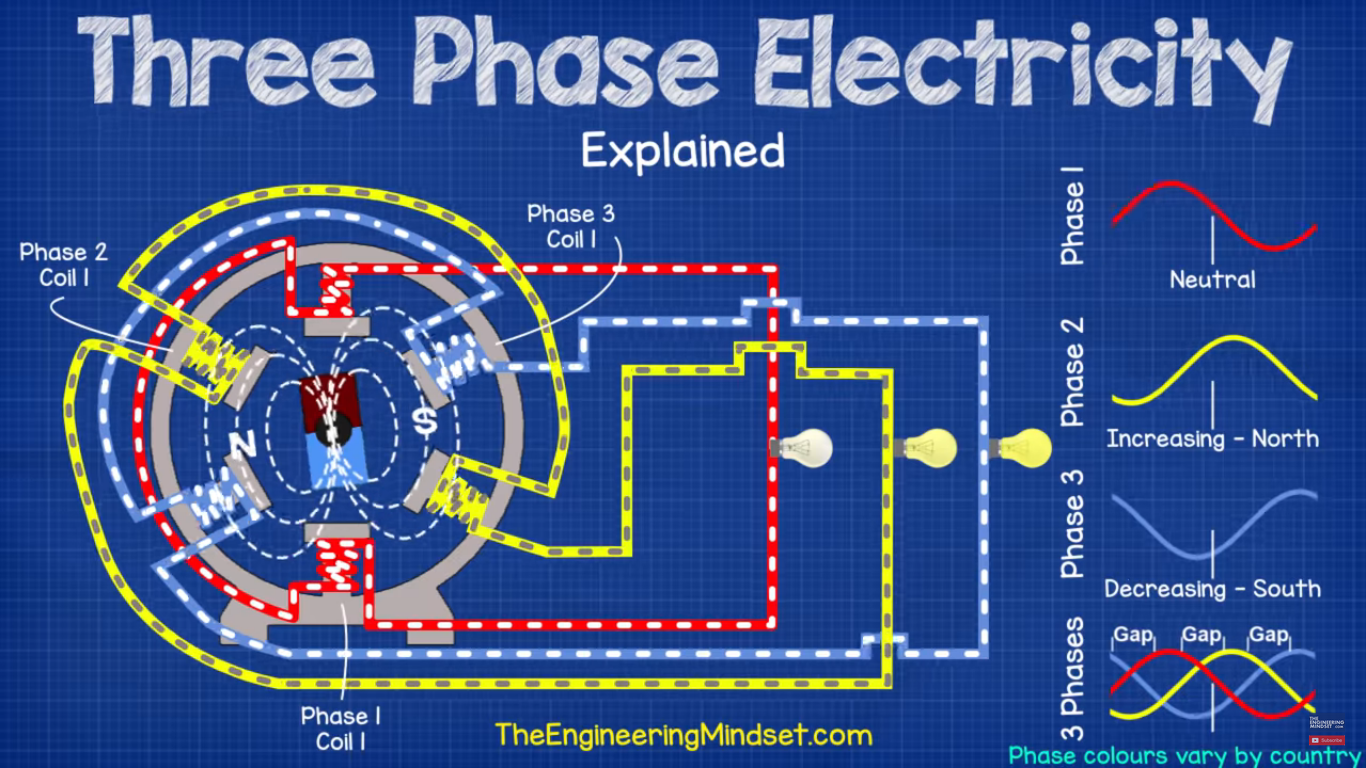
\includegraphics[width=16cm]{./images/EsquemaTrifasico.png}}
		\caption{Esquema de um Alternador Trifásico}
	\label{fig:alternador-trifasico}
\end{figure}


PRINT SCREEN DE https://youtu.be/4oRT7PoXSS0?t=345  em 5:45, acessado em 25/10/2018, 20:40

É possível, dada uma instalação trifásica, utilizar somente uma das fases em associação com o neutro para alimentar pequenos aparelhos, como lâmpadas e telas. Portanto, não é necessário ter duas redes elétricas dentro de uma mesma instalação industrial, por exemplo. Geralmente é desta maneira que energia elétrica é distribuída para residências, já que não espera-se que uma família tenha um forno industrial em sua cozinha.

\section{Sistemas Trifásico: Usos e Vantagens}

Como discutido acima, um sistema trifásico de transmissão (que se utiliza de três condutores) de energia possui diversas vantagens sobre sistemas monofásicos (que usam dois condutores). Dentre eles, o mais notório é o ganho em custo-benefício de tal sistema. Pode-se transmitir o triplo da energia com somente 50\% de incremento nos custos. A partir de 3 fases o incremento no custo é grande demais para compensar os benefícios.

Sistemas polifásicos são especialmente úteis e convenientes na construção e operação de motores elétricos, tal qual os motores de indução, por serem capazes de produzirem campos magnéticos rotativos de intensidades mais constantes e confiáveis. É possível alterar a frequência das três fases para alterar a velociade de rotação do motor, por exemplo. Motores de indução que utilizam corrente contínua requerem diversas peças adicionais, como transformadores, que encarecem o mecanismo final. Menores flutuações na potência entregue aos eixos também significa que menor stress será causado ao material, permitindo o uso de materiais mais baratos ou leves, aumentando ainda mais a eficiência e o custo-benefício.

De maneira análoga à motores de indução, sistemas de distribuição trifásicos são capazes de aproveitar mais da energia gerada por um gerador, como turbinas de uma hidrelétrica.

\section{Projeto: Identificador de Sinais Trifásicos}

Ao longo de grandes instalações elétricas, ao se utilizar modelos trifásicos, deve-se garantir que os diversos dispositivos e conexões estão ligados às fases adequadas. Erros desta natureza podem causar desde ineficiência do maquinário ligado até catastróficos acidentes. A fim de auxiliar na tarefa, propõe-se que seja construído um Identificador de Fase para Sinais Trifásicos.

Sabendo-se que dois condutores fazem parte de um mesmo sistema de transmissão trifásico ou rede de transmissão, o aparato deve ser capaz de fazer a leitura da frequência presente em um e compará-la à frequência do outro, indicando se há ou não defasagem entre ambos. Deve-se construir também um sistema que garanta a confiabilidade da leitura, indicando ao usuário quando o sinal lido anteriormente não é mais confiável. O aparato deve, também, mitigar variações momenâneas causadas pelo início da leitura, tal qual o repetido conecta-desconecta causado pelos imperceptíveis e repetidos choques, natural do contato inicial entre materiais duros, como o metal dos fios e a p.

O usuário, após acoplar o aparato a condutor, terá consigo uma amostra da fase obtido através de contadores internos. Ao comparar o conteúdo do aparato com a fase de outro condutor, este indicará se há adianto ou atraso de um terço de um período dosegundo em relação ao primeiro. Parte-se do pressuposto que ambos têm frequências iguais, já que são leituras em partes distintas de uma mesma rede ou linha de transmissão.

Pode-se utilizar o aparato para garantir a sincronia entre duas linhas de transmissão distindas, regulando a frequência e fase da corrente alternada que passa por uma delas.

%----------------Exemplo: insere figura-----------------------
%\begin{figure}[!htp]
%	\centering
%	\fbox{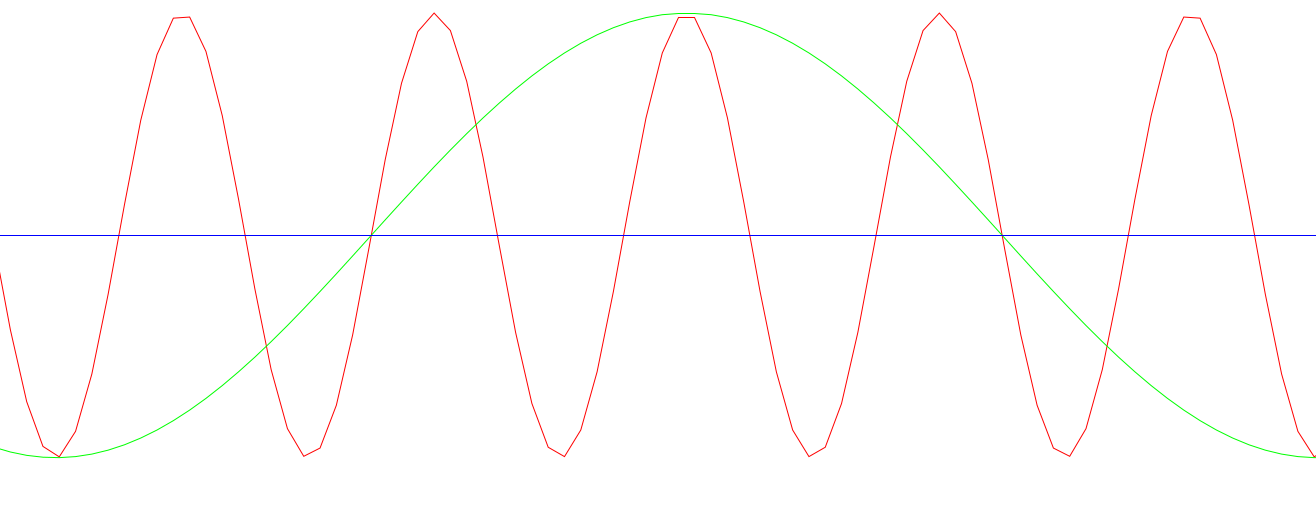
\includegraphics[width=16cm]{images/ondas.png}}
%		\caption{Exemplo de ondas sonoras}
%	\label{fig:ondas-sonoras}
%\end{figure}


%---------------Exemplo: insere tabela -----------------------
%\begin{table}[h]	
%	\centering	
%	\vspace{0.5cm}	
%\begin{tabular}{r|lr}
%Notas  & Frequ{\^e}ncia (Hz) \\
%\hline 
%C (Dó) & 261,33          \\
%D (Ré) & 293,66          \\
%E (Mi)  & 329,63 		 \\
%F (Fá)  & 349,23 		 \\
%G (Sol) & 391,99 		 \\  
%A (Lá)  & 440,00  		 \\
%B (Si)  & 493,88
%\end{tabular}
%	\label{tab:frequencia-notas}
%	\caption{Frequência da notas centrais do piano}
%\end{table}

\end{document}
